% Owner: E. M3b / H6 (rankings), input from results_function.tex.
% Values: results/e_summary.csv and results/e/m3b_*; figure: scripts/plot_e.py.
\begin{table}[t]
\centering
\small
\begin{tabular}{@{}llcc@{}}
\toprule
 & Measure & Real & P1 \\
\midrule
PS & $\tau$, unweighted & 0.71 & $0.55\pm0.01$ \\
   & $\tau$, weighted & 0.39 & $0.69\pm0.01$ \\
   & top-10\%, unweighted & 0.50 & $0.51\pm0.07$ \\
   & top-10\%, weighted & 0.29 & $0.60\pm0.06$ \\
\midrule
CM & $\tau$, unweighted & 0.78 & $0.85\pm0.00$ \\
   & $\tau$, weighted & 0.74 & $0.86\pm0.00$ \\
   & top-10\%, unweighted & 0.65 & $0.74\pm0.01$ \\
   & top-10\%, weighted & 0.57 & $0.72\pm0.02$ \\
\bottomrule
\end{tabular}
\caption{Agreement of static and temporal closeness rankings: Kendall $\tau_b$ and
overlap of the top 10\% nodes. P1: temporal closeness on 20 samples (mean $\pm$ sd); the
static ranking is unchanged by P1.}
\label{tab:m3b}
\end{table}

\begin{figure*}[t]
\centering
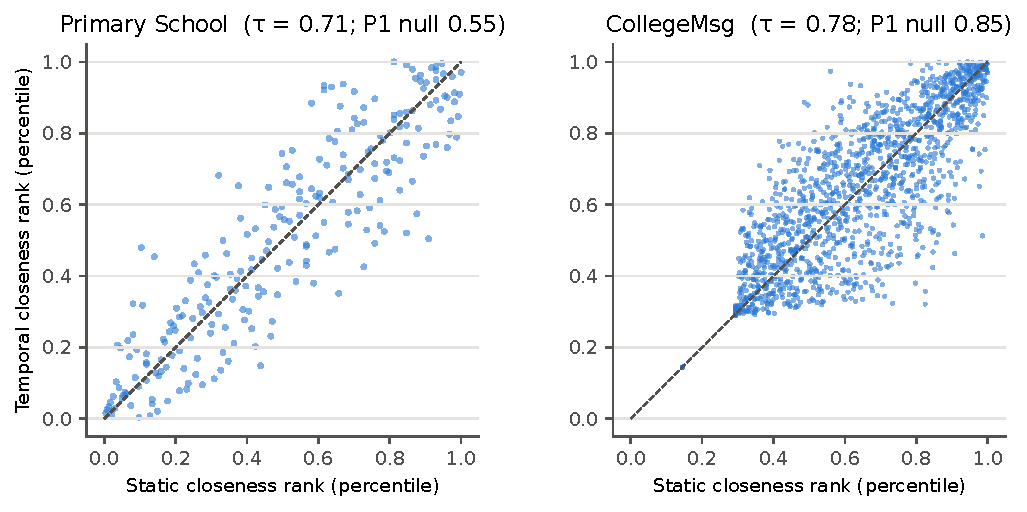
\includegraphics[width=0.8\linewidth]{e_m3b_rank_scatter.pdf}
\caption{Static (unweighted harmonic) vs.\ temporal closeness rank of every node; dashed:
identical rankings. The tied block at the lower left of the CM panel is the 29\% of users
who never send a message.}
\label{fig:m3b}
\end{figure*}

\paragraph{Centrality.}
Static and temporal closeness rankings are clearly correlated in both networks
(\cref{tab:m3b,fig:m3b}; $\tau=0.71$ in PS and $0.78$ in CM, hop distance), so the static
network shows roughly which nodes are central. It is much less reliable about which nodes
are \emph{most} central: only half of the PS top 10\% and two thirds of the CM top 10\%
coincide. In CM the real agreement is somewhat lower than under P1 (0.78 vs.\ 0.85), so
event order makes static closeness a slightly worse guide. The CM $\tau$ is also helped by
the 549 users (29\%) who never send a message and have zero closeness in both rankings
(the tied block in \cref{fig:m3b}).

In PS the effect depends on edge weights. Weighted static closeness agrees poorly with
temporal closeness ($\tau=0.39$, top-10\% overlap 0.29), whereas after P1 the agreement
is high ($0.69\pm0.01$). In the school, most contact weight comes from repeated contacts
within a class during lessons; these happen while the class is already connected and
hardly shorten time-respecting paths to the rest of the school. Under P1 the same contacts
are spread over the day, and a heavy edge becomes a frequent chance to transmit. Without
weights the effect reverses (real 0.71 vs.\ P1 0.55): reaching the school quickly depends
on having many distinct partners, which in PS largely means mixing at breaks.

\emph{Rankings part of H6: partly supported.} The rankings are correlated
($\tau=0.71$--$0.78$) but the top nodes differ by 35--50\%, and in face-to-face data
weighting edges by contact frequency makes the static ranking misleading ($\tau=0.39$).
